\documentclass{article}
\usepackage[UTF8]{ctex}
\usepackage{geometry}
\usepackage{listings}
\usepackage{fancyhdr}
\usepackage[colorlinks,linkcolor=black]{hyperref} 

%\usepackage{amsmath}
\usepackage{graphicx}
%\usepackage{pgfplots}

\geometry{left = 2cm,right = 2cm,top = 3cm,bottom = 3cm}
\pagestyle{fancy}
\fancyhf{}
\fancyhead[R]{\leftmark}
\fancyhead[L]{\rightmark}
\fancyhead[C]{多周期处理器}
\fancyfoot[C]{\thepage}
\renewcommand{\headrulewidth}{0.2mm}

\title{数字逻辑与处理器基础\\多周期处理器}

\author{cvxbzn}

\begin{document}

\maketitle
\tableofcontents
\newpage
\section{数据通路设计}
\subsection{寄存器与多路选择器及其功能}
\begin{itemize}
    \item 寄存器
          \begin{itemize}
              \item PC:输入下一状态PC,输出当前PC,使能信号为1时在时钟上升沿写入。
              \item 指令寄存器(IR):存放从存储器中取出的指令,IRWrite为1时在时钟上升沿写入
              \item 数据寄存器(MDR):输入存储器的输出MemData。
              \item 临时寄存器A:输入为寄存器堆中的ReadData1
              \item 临时寄存器B:输入为寄存器堆中的ReadData2
              \item ALU寄存器ALUOut:存放ALU输出ALUOut
          \end{itemize}
    \item 多路选择器
          \begin{itemize}
              \item IorD:Instruction or data,选择读取存储器的数据为指令(0)或者数据(1)。
              \item RegDst:选择写回寄存器堆中的寄存器位置,rt(00),rd(01)或者\$ra(10),其中\$ra在执行jal指令时使用。
              \item MemToReg:选择写回寄存器堆的数据来源。ALUOut(00),内存数据(01),PC(10)。
              \item ALUSrcA:选择ALU操作数1的数据来源,PC(00),临时寄存器A(01),以及在移位时用到的Shamt(10)
              \item ALUSrcB:选择ALU操作数2的数据来源,临时寄存器B(00),常数4(01),立即数(10)以及移位后的立即数(11)
              \item PCSource:选择更新PC时PC的来源,PC+4(00),分支指令计算结果(01)以及伪直接寻址(10)
          \end{itemize}
\end{itemize}
具体情况如下示意图所示,代码见附件。
\subsection{示意图}
\begin{center}

\end{center}

\section{控制信号分析与有限状态机实现}
\subsection{控制信号及具体功能}
\begin{itemize}
    \item PCWrite:PC 寄存器的写使能信号;0-不能写 PC;1-允许写 PC
    \item PCWriteCond:分支指令PC写使能信号,0-无分支指令;1-有分支指令
    \item IorD:选择读取存储器的数据信号,0-指令,1-数据
    \item MemWrite:内存的写使能信号;0-不能写内存;1-允许写内存
    \item MemRead:内存的读使能信号;0-不能读内存;1-允许读内存
    \item IRWrite:指令寄存器的写使能信号;0-不能写;1-允许写
    \item MemToReg:写回寄存器堆数据来源选择信号;00-ALUOut,01-内存数据,10-PC
    \item RegDst:写回寄存器堆的寄存器位置选择信号,00-rt,01-rd或者10-\$ra
    \item RegWrite:寄存器堆的写使能信号;0-不能写;1-允许写
    \item ExtOp:符号扩展信号,0-逻辑扩展;1-算术扩展
    \item LuiOp:Lui控制信号,0-不左移16位;1-左移16位
    \item ALUSrcA:ALU操作数1数据来源选择信号;00-PC;01-临时寄存器A;10-Shamt
    \item ALUSrcB:ALU操作数2数据来源选择信号;00-临时寄存器B;01-常数4;10-立即数;11-移位后的立即数
    \item ALUOp:ALU控制信号;000-ADD;001-SUB;100-AND;101-SLT;010-取决于Funct
    \item PCSource:PC更新来源选择信号;00-PC+4;01-分支指令计算结果;10-伪直接寻址
\end{itemize}
\subsection{状态转移图}
\begin{center}
    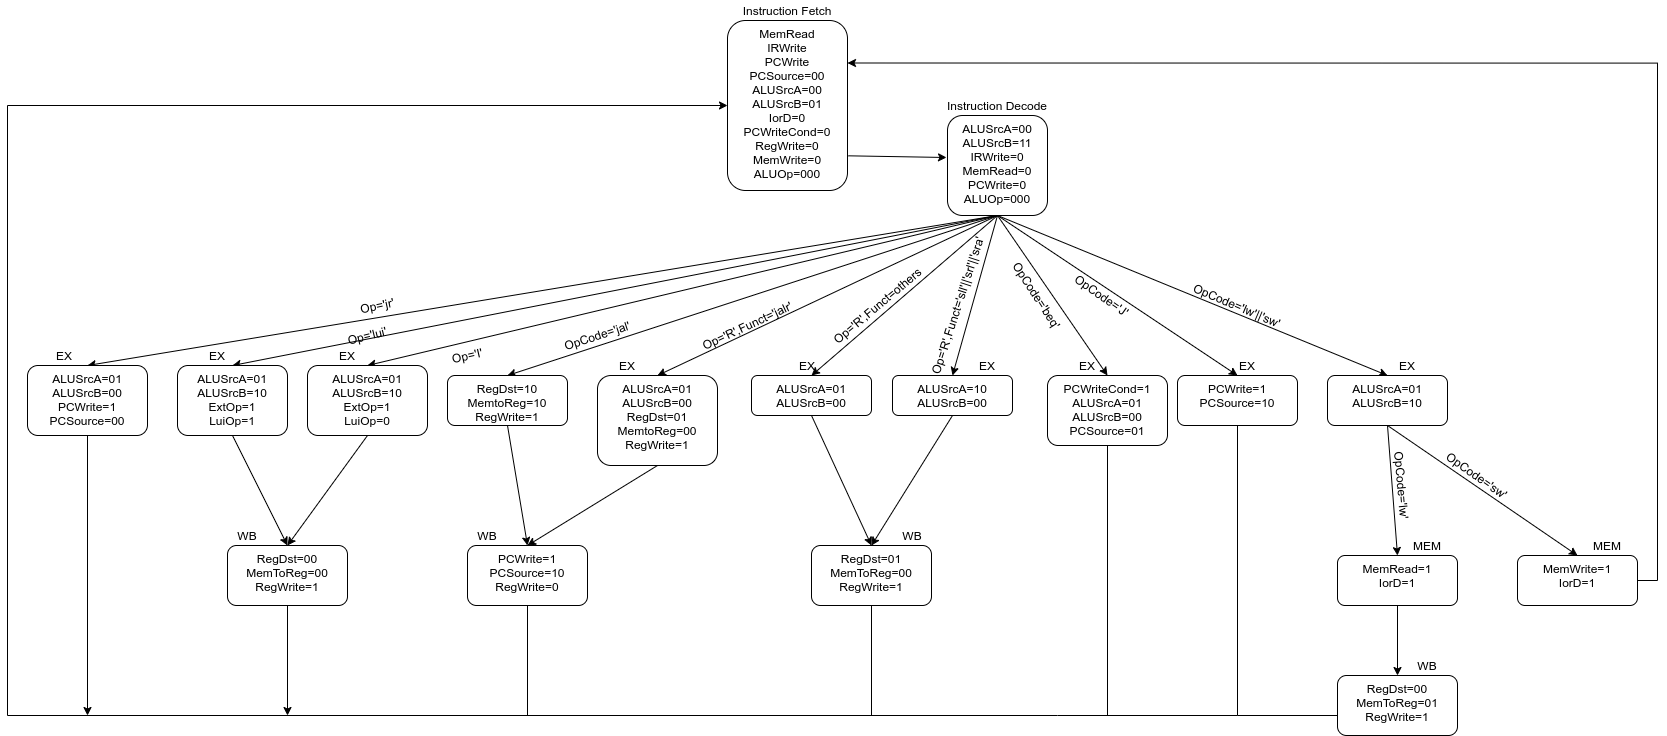
\includegraphics[width = 18cm]{images/fsm.png}
\end{center}


\section{ALU功能拓展}
\subsection{setsub类型和机器码字段内容}
setsub rd rs rt : \{6'h0,rs[4:0],rt[4:0],rd[4:0],5'h0,6'h28\}
\subsection{ALU verilog代码修改}
对应ALUConf设置为5'b00011,设计执行程序为
\begin{lstlisting}
    lui $a0 0xABCD      
    addi $a0 $a0 0x1234  
    lui $a1 0xCDEF
    addi $a1 $a1 0x3456  
    setsub $a2 $a0 $a1
    Loop:
    beq $zero $zero Loop
\end{lstlisting}
对应机器码为
\begin{lstlisting}
    {6'h0f,5'd0,5'd4,16'habcd}
    {6'h08,5'd4,5'd4,16'h1234}
    {6'h0f,5'd0,5'd5,16'hcdef}
    {6'h08,5'd5,5'd5,16'h3456}
    {6'h0,5'd4,5'd5,5'd6,5'h0,6'h28}
    {6'h04,5'd0,5'd0,16'hffff}
\end{lstlisting}
具体代码见附件。
\subsection{仿真结果}
0xabcd1234 setsub 0xcdef5678  \\
= 1010\_1011\_1100\_1101\_0001\_0010\_0011\_0100 setsub 1100\_1101\_1110\_1111\_0011\_0100\_0101\_0110\\
= 0010\_0010\_0000\_0000\_0000\_0010\_0010\_0000 = 0x2200\_0220\\
仿真结果如图
\begin{center}
    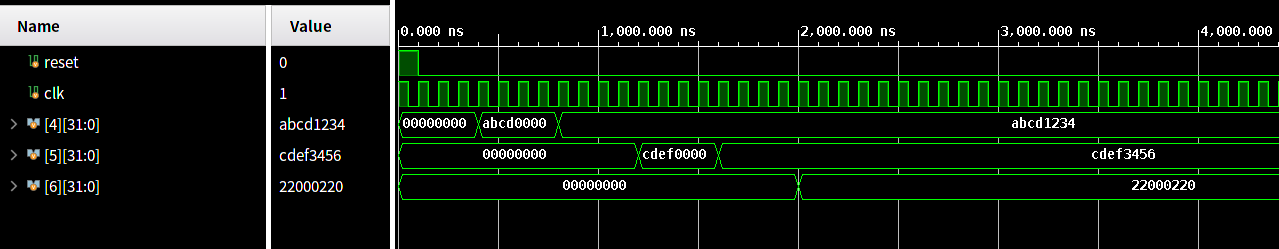
\includegraphics[width = 16cm]{images/sim_setsub_waveform.png}
\end{center}
与预期一致。

\section{汇编程序分析-1}
\subsection{计算寄存器值}
\begin{lstlisting}
    addi $a0, $zero, 12123      # $a0 = 0x0000_2f5b
    addiu $a1, $zero, -12345    # $a1 = 0xffff_cfc7
    sll $a2, $a1, 16            # $a2 = 0xcfc7_0000
    sra $a3, $a2, 16            # $a3 = 0xffff_cfc7
    beq $a3, $a1, L1            # 跳转至L1
    lui $a0, 22222              # 不执行

    L1:
    add $t0, $a2, $a0           # $t0 = 0xcfc7_2f5b
    sra $t1, $t0, 8             # $t1 = 0xffcf_c72f
    addi $t2, $zero, -12123     # $t2 = 0xffff_d0a5
    slt $v0, $a0, $t2           # 有符号情况下 $a0 > $t2 ,$v0=1
    sltu $v1, $a0, $t2          # 无符号情况下 $a0 < $t2 ,$v1=0

    Loop:
    j Loop
\end{lstlisting}
\subsection{仿真结果}
\begin{center}
    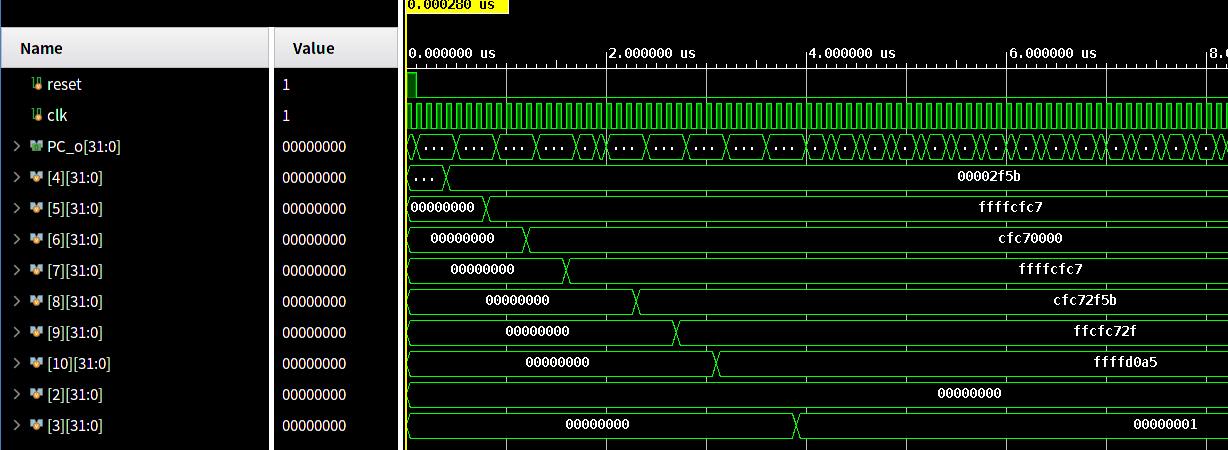
\includegraphics[width = 16cm]{images/sim_1_waveform.png}
\end{center}
可见与计算结果一致。

\section{汇编程序分析-2}
\subsection{程序功能以及代码注释}
\begin{lstlisting}
    addi $a0, $zero, 5      # $a0 = 5
    xor $v0, $zero, $zero   # $v0 = 0
    jal sum                 # 跳转到sum
    Loop:
    beq $zero, $zero, Loop  # 程序结束
    sum:
    addi $sp, $sp, -8       # 入栈前栈指针-8
    sw $ra, 4($sp)          # $ra 入栈
    sw $a0, 0($sp)          # $a0 入栈
    slti $t0, $a0, 1        # if $a0 < 1 $t0 = 1
    beq $t0, $zero, L1      # if $a0 >= 1, goto L1
    addi $sp, $sp, 8        # 出栈恢复栈指针
    jr $ra                  # 回到上一个过程$ra存的位置
    L1:
    add $v0, $a0, $v0       # $v0 = $a0 + $v0
    addi $a0, $a0, -1       # $a0 = $a0 - 1
    jal sum                 # 迭代
    lw $a0, 0($sp)          
    lw $ra, 4($sp)
    addi $sp, $sp, 8        # 出栈恢复栈指针
    add $v0, $a0, $v0       # 又加一次,$v0 = $a0 + $v0
    jr $ra
\end{lstlisting}
可见每次循环相当于加了两次\$a0,因此如果第一行的 5 是任意正整数 n,程序实现了2$\sum_{i=1}^ni$的功能。此外由于lw,\$a0最终值仍为n。
\subsection{将汇编翻译成机器码并写出}
\begin{lstlisting}
    {6'h08,5'd0,5'd4,16'd5}
    {6'h0,5'd0,5'd0,5'd2,5'h0,6'h26}
    {6'h03,26'd4}
    {6'h04,5'd0,5'd0,16'hffff}
    {6'h08,5'd29,5'd29,16'dfff8}
    {6'h2b,5'd29,5'd31,16'd4}
    {6'h2b,5'd29,5'd4,16'd0}
    {6'h0a,5'd4,5'd8,16'd1}
    {6'h04,5'd8,5'd0,16'd2}
    {6'h08,5'd29,5'd29,16'd8}
    {6'h0,5'd31,15'd0,6'h08}
    {6'h0,5'd4,5'd2,5'd2,5'd0,6'h20}
    {6'h08,5'd04,5'd04,16'hffff}
    {6'h03,26'h4}
    {6'h23,5'd29,5'd4,16'd0}
    {6'h23,5'd29,5'd31,16'd4}
    {6'h08,5'd29,5'd29,16'd8}
    {6'h0,5'd4,5'd2,5'd2,5'd0,6'h20}
    {6'h0,5'd31,15'd0,6'h08}
\end{lstlisting}
修改文件位于InstAndDataMemory\_1.v
\subsection{\$a0,\$v0值}
根据上述分析,\$v0值为30,即0x1e,\$a0值为5,仿真结果如图
\begin{center}
    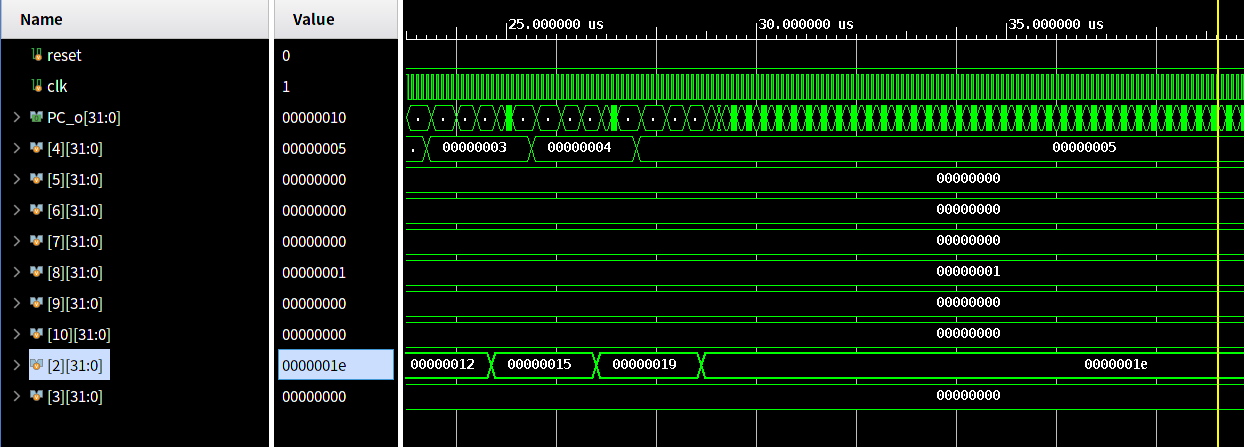
\includegraphics[width = 16cm]{images/sim_2_waveform.png}
\end{center}

\subsection{观察、描述并解释寄存器如何变化}
PC在sIF状态结束时+4,在beq、j、jal、jr的EX阶段结束时PC跳转到对应的地址,如下图所示。
\begin{center}
    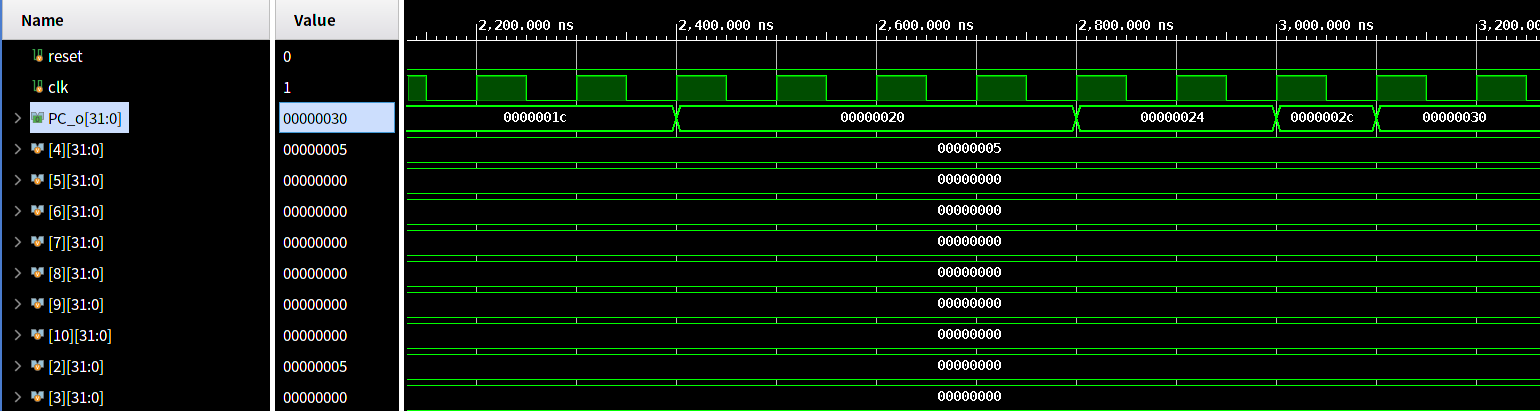
\includegraphics[width = 16cm]{images/pc_waveform.png}
\end{center}
\$a0从5减小至0再增加至0,
\begin{lstlisting}
    addi $a0, $a0, -1
\end{lstlisting}
使\$a0减小,减至0后lw指令装载之前\$a0值。\\
\$v0是\$a0累加,
\[\$v0 = 5+4+3+2+1+1+2+3+4+5\]
入栈时\$sp减8,当\$a0等于0时开始出栈,\$sp加8。\\
\$ra在执行jal指令时改变,第一次jal时\$ra为0x0c,之后为0x38,最后一次lw后\$ra为0x0c。

\section{异常处理}
\subsection{控制信号与功能}
\begin{itemize}
    \item exp\_flag:异常判断信号,0-无异常,1-异常
    \item exp\_write:异常寄存器(EPC,ErrorTarget)写信号,0-不能写,1-允许写
    \item exp\_state:异常PC跳转选择信号,0-0x7c,1-EPC
\end{itemize}
\subsection{指令格式与状态转移图}
由于异常处理程序只涉及将0xffff\_ffff写回目标寄存器无额外功能,因此只需要分配新OpCode加以区分。指令格式
\begin{lstlisting}
    {6'h05,26'h0}
\end{lstlisting}
状态转移图为
\begin{center}
    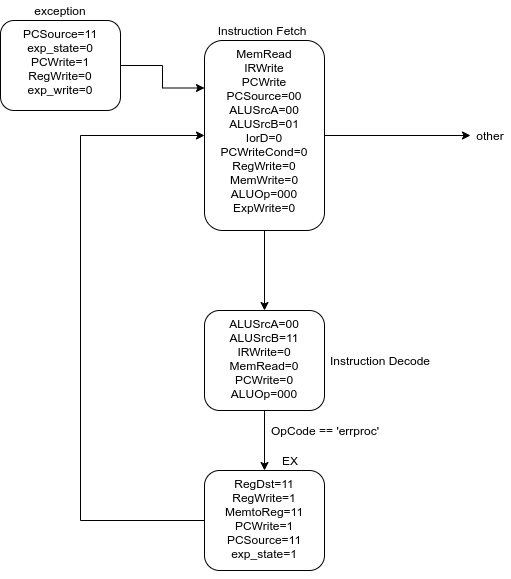
\includegraphics[width = 12cm]{images/exception_fsm.png}
\end{center}
\subsection{仿真}
汇编程序为
\begin{lstlisting}
    lui $a0 0x7fff
    addi $a0 $a0 0x1234
    lui $a1 0x7fff
    addi $a1 $a1 0x1234
    add $a0 $a0 $a1
    addi $a2 $0 5
    addi $a2 $a2 4
    Loop:
    beq $zero $zero Loop
\end{lstlisting}
对应机器码为
\begin{lstlisting}
    {6'h0f,5'd0,5'd4,16'h7fff}
    {6'h08,5'd4,5'd4,16'h1234}
    {6'h0f,5'd0,5'd5,16'h7fff}
    {6'h08,5'd5,5'd5,16'h1234}
    {6'h0,5'd4,5'd5,5'd4,5'h0,6'h20}
    {6'h08,5'd0,5'd6,16'd5}
    {6'h08,5'd6,5'd6,16'd4}
    {6'h04,5'd0,5'd0,16'hffff}
\end{lstlisting}
程序写在InstAndDataMemory\_exp.v中,需修改顶层文件对应模块名称。这段程序\$a0会溢出,最终值应为ffff\_ffff,而\$a2继续执行,最终值应为9。\\
仿真结果为
\begin{center}
    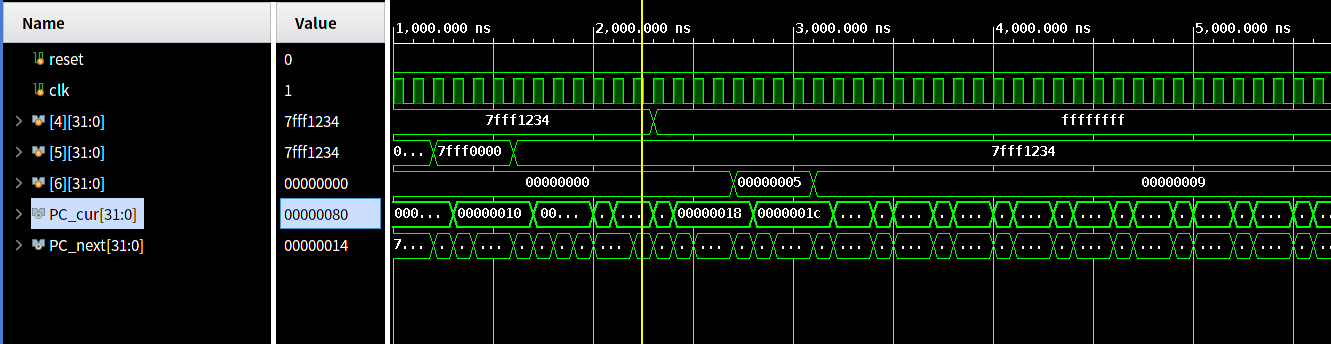
\includegraphics[width = 16cm]{images/sim_exp_waveform.png}
\end{center}
与预期一致。
%\begin{lstlisting}[language=Matlab]
%\end{lstlisting}

\end{document}